%%%%%%%%%%%%%%%%%%%%%%%%%%%%%%%%%%%%%%%%%%%%%%%%%%%%%%%%%%%%%%%%%%%%%%%%%%%%%%%%
\section{Our Task}
{   
	\usebackgroundtemplate{
		\vbox to \paperheight{\vfil\hbox to \paperwidth{\hfil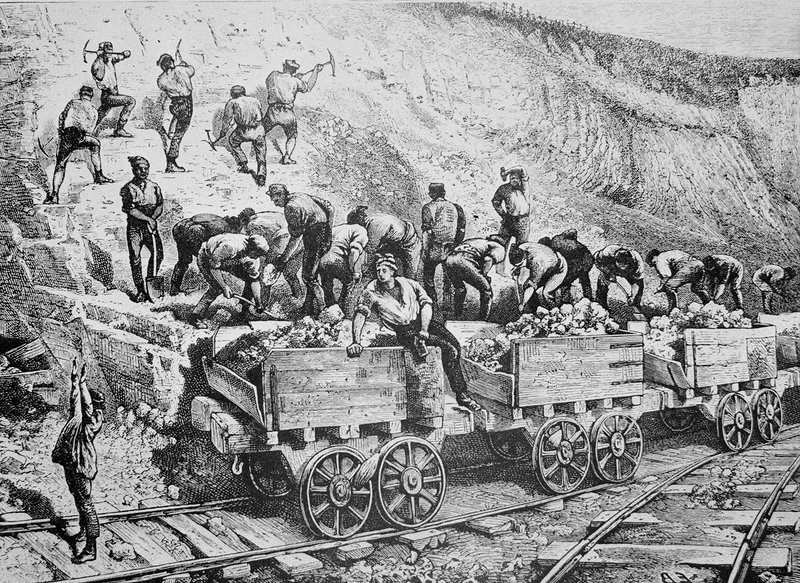
\includegraphics[height=\paperheight]{Railway_construction,_19th_century.jpg}\hfil}\vfil}
		%https://www.flaticon.com/free-icon/decoration_2788716
		%<a href="https://www.flaticon.com/free-icons/decoration" title="decoration icons">Decoration icons created by Freepik - Flaticon</a>
		
	}
	\frame{
		\frametitle{Let's get started}
		\begin{mdframed}[tikzsetting={draw=white,fill=white,fill opacity=0.8,
				line width=0pt},backgroundcolor=none,leftmargin=0,
			rightmargin=150,innertopmargin=4pt,roundcorner=10pt]
			\tableofcontents[currentsection,sections={1-5},hideothersubsections]
		\end{mdframed}
	}
}

%%%%%%%%%%%%%%%%%%%%%%%%%%%%%%%%%%%%%%%%%%%%%%%%%%%%%%%%%%%%%%%%%%%%%%%%%%%%%%%%
\begin{frame}
	\frametitle{Our Task \ldots}
	\ldots
	is simple. We are going to
	\begin{itemize}
		\item convert degrees of Fahrenheit into Celsius using $\circ\mathsf{C} = \frac{\circ\mathsf{F} - 32}{1.8}$
		\item estimate the value of $\pi$ by throwing darts in a circle.
	\end{itemize}
    Our code is broken and we fill see this using a CI pipeline!
    \pause
    \begin{question}[Is this too simple?]
    	{In real RSE, we are frequently dealing with little bugs, i.\,e. a wrong digit, a false memory access, etc.}
    \end{question}
\end{frame}

%%%%%%%%%%%%%%%%%%%%%%%%%%%%%%%%%%%%%%%%%%%%%%%%%%%%%%%%%%%%%%%%%%%%%%%%%%%%%%%%
\begin{frame}
	\frametitle{\HandsOn{Forking a Repository}}
	\begin{block}{Background}
		{Forking repos is the first step fixing a software, if you are not a team member of that project.}
	\end{block}
	\pause
	\begin{columns}
		\begin{column}{0.5\textwidth}
			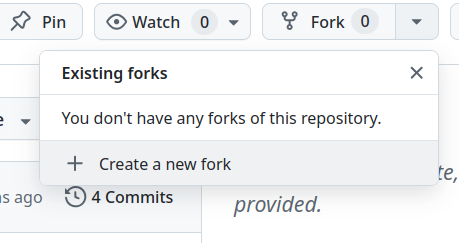
\includegraphics[width=0.9\textwidth]{fork.png}
		\end{column}
		\begin{column}{0.5\textwidth}
			Please fork the repo \url{https://github.com/cmeesters/ci-exercises}.
		\end{column}
	\end{columns}
\end{frame}

%%%%%%%%%%%%%%%%%%%%%%%%%%%%%%%%%%%%%%%%%%%%%%%%%%%%%%%%%%%%%%%%%%%%%%%%%%%%%%%%
\begin{frame}[fragile]
	\frametitle{\HandsOn{Pulling a Repository}}
	So, you just forked a repo as your "own" fork. This is how you get it locally.
	\begin{lstlisting}[language=Bash, style=Shell,escapeinside={(*}{*)}]
$ git clone git(*@*)github.com:<username>/ci-exercises
	\end{lstlisting}
    Afterwards your repo should look like (plus some files):

\centering
\begin{minipage}[t]{0.8\textwidth}
	\setstretch{0.1}
	{\tiny \DTsetlength{0.2em}{1em}{0.2em}{0.4pt}{.6pt}
		\dirtree{%
			.1 {CMakeLists.txt}.
			.1 {pyproject.toml}.
			.1 {environment.yaml}.
			.1 {src}.
			.2 {converter.py}.
			.2 {\ldots}.
			.2 {pi\_estimator.cpp}.
			.2 {tests}.
			.3 {test\_converter.py}.
			.3 {test\_pi\_estimator.cpp}.
	}}
\end{minipage}
\end{frame}

%%%%%%%%%%%%%%%%%%%%%%%%%%%%%%%%%%%%%%%%%%%%%%%%%%%%%%%%%%%%%%%%%%%%%%%%%%%%%%%%
\begin{frame}<handout:0>[fragile]
	\frametitle{Activating the Conda Environment}
	\begin{lstlisting}[language=Bash, style=Shell]
$ conda activate ci-exercises
    \end{lstlisting}
\end{frame}

%%%%%%%%%%%%%%%%%%%%%%%%%%%%%%%%%%%%%%%%%%%%%%%%%%%%%%%%%%%%%%%%%%%%%%%%%%%%%%%%
\begin{frame}[fragile]
	\frametitle{Running Tests locally (Python)}
	\begin{warning}[The Importance of local Testing]
		{By running tests locally, you can avoid being surprised during the CI run and can fix code \emph{before} pushing to the git origin.}
	\end{warning}
    \pause
    \begin{lstlisting}[language=Bash, style=Shell]
$ # to test the python code
$ poetry run pytest tests/
$ # to produce a coverage report run
$ poetry run coverage run -m pytest tests/
$ poetry run coverage report
    \end{lstlisting}	
\end{frame}



%%%%%%%%%%%%%%%%%%%%%%%%%%%%%%%%%%%%%%%%%%%%%%%%%%%%%%%%%%%%%%%%%%%%%%%%%%%%%%%%
\begin{frame}
	\frametitle{\HandsOn{Something is broken \ldots}}
	\ldots but we are not going to fix this, now!
	\begin{question}
	  {Do you find the error in the conversion function?}
	\end{question}
\end{frame}

%%%%%%%%%%%%%%%%%%%%%%%%%%%%%%%%%%%%%%%%%%%%%%%%%%%%%%%%%%%%%%%%%%%%%%%%%%%%%%%%
\begin{frame}[fragile]
	\frametitle{Running Tests locally (\CC)}
	\begin{warning}[The Importance of local Testing]
		{By running tests locally, you can avoid being surprised during the CI run and can fix code \emph{before} pushing to the git origin. With compiled languages, you can first compile locally and then run a test suite. Usually, the compilation gives sufficient error message. Not here, though \ldots}
	\end{warning}
	\pause
	\begin{lstlisting}[language=Bash, style=Shell]
$ cmake CMakeLists.txt
$ make
$ # this builds a program AND test suite
$ # 1st run the program with different inputs
$ ./pi_estimator 10 or 100 or 1000000  
$ ./pi_estimator_test    # then the test
	\end{lstlisting}	
\end{frame}

%%%%%%%%%%%%%%%%%%%%%%%%%%%%%%%%%%%%%%%%%%%%%%%%%%%%%%%%%%%%%%%%%%%%%%%%%%%%%%%%
\begin{frame}
	\frametitle{\HandsOn{Something is broken \ldots}}
	\ldots but we are not going to fix this, now!
	\begin{question}
		{Do you find the error in the code?}
	\end{question}
\end{frame}

%%%%%%%%%%%%%%%%%%%%%%%%%%%%%%%%%%%%%%%%%%%%%%%%%%%%%%%%%%%%%%%%%%%%%%%%%%%%%%%%
\begin{frame}<handout:0>
	\frametitle{What we are NOT covering}
	\begin{warning}[Unittests]
		{In this course, we are not going into the coding of unittests, the different test frameworks etc.\\
			There are different libraries for the various languages and projects.}
	\end{warning}
	\pause
	\begin{block}{Up to You}
		{If you want to we can take a \emph{brief look} into the unittest codes for this workshop -- NOW.}
	\end{block}	
\end{frame}
